% Options for packages loaded elsewhere
\PassOptionsToPackage{unicode}{hyperref}
\PassOptionsToPackage{hyphens}{url}
%
\documentclass[
]{article}
\usepackage{amsmath,amssymb}
\usepackage{lmodern}
\usepackage{ifxetex,ifluatex}
\ifnum 0\ifxetex 1\fi\ifluatex 1\fi=0 % if pdftex
  \usepackage[T1]{fontenc}
  \usepackage[utf8]{inputenc}
  \usepackage{textcomp} % provide euro and other symbols
\else % if luatex or xetex
  \usepackage{unicode-math}
  \defaultfontfeatures{Scale=MatchLowercase}
  \defaultfontfeatures[\rmfamily]{Ligatures=TeX,Scale=1}
\fi
% Use upquote if available, for straight quotes in verbatim environments
\IfFileExists{upquote.sty}{\usepackage{upquote}}{}
\IfFileExists{microtype.sty}{% use microtype if available
  \usepackage[]{microtype}
  \UseMicrotypeSet[protrusion]{basicmath} % disable protrusion for tt fonts
}{}
\makeatletter
\@ifundefined{KOMAClassName}{% if non-KOMA class
  \IfFileExists{parskip.sty}{%
    \usepackage{parskip}
  }{% else
    \setlength{\parindent}{0pt}
    \setlength{\parskip}{6pt plus 2pt minus 1pt}}
}{% if KOMA class
  \KOMAoptions{parskip=half}}
\makeatother
\usepackage{xcolor}
\IfFileExists{xurl.sty}{\usepackage{xurl}}{} % add URL line breaks if available
\IfFileExists{bookmark.sty}{\usepackage{bookmark}}{\usepackage{hyperref}}
\hypersetup{
  pdftitle={Rotinas do Ambulatório de Uroginecologia},
  pdfauthor={Dr.~Ricardo José de Souza},
  hidelinks,
  pdfcreator={LaTeX via pandoc}}
\urlstyle{same} % disable monospaced font for URLs
\usepackage[margin=1in]{geometry}
\usepackage{graphicx}
\makeatletter
\def\maxwidth{\ifdim\Gin@nat@width>\linewidth\linewidth\else\Gin@nat@width\fi}
\def\maxheight{\ifdim\Gin@nat@height>\textheight\textheight\else\Gin@nat@height\fi}
\makeatother
% Scale images if necessary, so that they will not overflow the page
% margins by default, and it is still possible to overwrite the defaults
% using explicit options in \includegraphics[width, height, ...]{}
\setkeys{Gin}{width=\maxwidth,height=\maxheight,keepaspectratio}
% Set default figure placement to htbp
\makeatletter
\def\fps@figure{htbp}
\makeatother
\setlength{\emergencystretch}{3em} % prevent overfull lines
\providecommand{\tightlist}{%
  \setlength{\itemsep}{0pt}\setlength{\parskip}{0pt}}
\setcounter{secnumdepth}{-\maxdimen} % remove section numbering
\ifluatex
  \usepackage{selnolig}  % disable illegal ligatures
\fi
\newlength{\cslhangindent}
\setlength{\cslhangindent}{1.5em}
\newlength{\csllabelwidth}
\setlength{\csllabelwidth}{3em}
\newenvironment{CSLReferences}[2] % #1 hanging-ident, #2 entry spacing
 {% don't indent paragraphs
  \setlength{\parindent}{0pt}
  % turn on hanging indent if param 1 is 1
  \ifodd #1 \everypar{\setlength{\hangindent}{\cslhangindent}}\ignorespaces\fi
  % set entry spacing
  \ifnum #2 > 0
  \setlength{\parskip}{#2\baselineskip}
  \fi
 }%
 {}
\usepackage{calc}
\newcommand{\CSLBlock}[1]{#1\hfill\break}
\newcommand{\CSLLeftMargin}[1]{\parbox[t]{\csllabelwidth}{#1}}
\newcommand{\CSLRightInline}[1]{\parbox[t]{\linewidth - \csllabelwidth}{#1}\break}
\newcommand{\CSLIndent}[1]{\hspace{\cslhangindent}#1}

\title{Rotinas do Ambulatório de Uroginecologia}
\usepackage{etoolbox}
\makeatletter
\providecommand{\subtitle}[1]{% add subtitle to \maketitle
  \apptocmd{\@title}{\par {\large #1 \par}}{}{}
}
\makeatother
\subtitle{Hospital Universitário Pedro Ernesto - UERJ}
\author{Dr.~Ricardo José de Souza}
\date{versão 2021.1}

\begin{document}
\maketitle

\hypertarget{via-de-acesso-ao-ambulatuxf3rio}{%
\subsubsection{\texorpdfstring{\textbf{Via de acesso ao
ambulatório}:~}{Via de acesso ao ambulatório:~}}\label{via-de-acesso-ao-ambulatuxf3rio}}

\begin{itemize}
\item
  Via SISREG ou SER (03 vagas); ou
\item
  Via encaminhamento interno de mulheres já atendidas por outras
  clínicas no HUPE ou PPC.
\end{itemize}

\hypertarget{perfil-do-paciente}{%
\subsubsection{\texorpdfstring{\textbf{Perfil do
paciente:}}{Perfil do paciente:}}\label{perfil-do-paciente}}

\begin{itemize}
\item
  Prolapso genital;
\item
  Incontinência urinária associada a prolapso;
\item
  Infecções urinárias de repetição;
\item
  Dor pélvica crônica associada a sintomas urinários ou prolapsos; e
\item
  Fístula vesico-vaginal.
\end{itemize}

\hypertarget{atendimento-da-paciente-no-ambulatuxf3rio-primeira-consulta}{%
\subsubsection{\texorpdfstring{\textbf{Atendimento da paciente no
Ambulatório Primeira
consulta:}}{Atendimento da paciente no Ambulatório Primeira consulta:}}\label{atendimento-da-paciente-no-ambulatuxf3rio-primeira-consulta}}

As pacientes devem ser inseridas no banco de dados criado para o
ambulatório (Projeto prolapso), através do endereço do REDCap via web:
\href{http://www.redcap.lampada.uerj.br}{ww.redcap.lampada.uerj.br}.
Todos os itens abaixo devem ser preenchidos na primeira consulta:

\begin{itemize}
\item
  Cadastro;
\item
  Anamnese;
\item
  Exame físico;
\item
  Tratamento proposto; e
\item
  Questionários de autopreenchimento (são entregues às pacientes pela
  recepcionista e preenchidas antes da consulta):

  \begin{itemize}
  \item
    Questionário de impacto no assoalho pélvico (PFIQ-7);
  \item
    Questionário de incontinência urinária (ICIQ-SF); e
  \item
    Questionário de qualidade do sono.
  \end{itemize}
\end{itemize}

Após inserir todos as informações no banco de dados, preencher o
prontuário eletrônico (MV) com as informações importantes da consulta
(lembrar que nem todos terão acesso ao REDCap, pois este é apenas para
fins de pesquisa):

Anamnese;

\begin{itemize}
\item
  HPP;
\item
  HGO;
\item
  Exame físico; e
\item
  Tratamento proposto.
\end{itemize}

\hypertarget{pacientes-com-indicauxe7uxe3o-ciruxfargica}{%
\paragraph{\texorpdfstring{\textbf{Pacientes com indicação
cirúrgica:}}{Pacientes com indicação cirúrgica:}}\label{pacientes-com-indicauxe7uxe3o-ciruxfargica}}

\begin{itemize}
\item
  Solicitar exames pré-operatórios;
\item
  Inserir na fila de cirurgias do serviço (\emph{Google forms});
\item
  Explicar para a paciente os detalhes da cirurgia indicada e
  \textbf{entregar o consentimento informado} (a paciente deve levar
  para casa preenchido e assinado pelo médico, em duas vias, e trazer no
  dia da internação assinado).
\end{itemize}

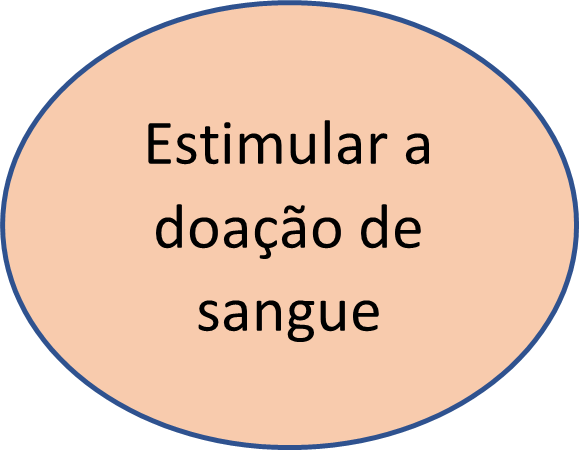
\includegraphics[width=2.30208in,height=1.28125in]{Imagem1.png}

\hypertarget{durante-a-internauxe7uxe3o-ciruxfargica}{%
\paragraph{\texorpdfstring{\textbf{Durante a internação
cirúrgica:}}{Durante a internação cirúrgica:}}\label{durante-a-internauxe7uxe3o-ciruxfargica}}

Verificar \textbf{se assinou o} \textbf{consentimento informado}
(entregue durante a consulta do ambulatório) e anexar ao prontuário;

Pacientes submetidas a cirurgia (preencher no
\href{www.redcap.lampada.uerj.br}{REDCap}):

\begin{itemize}
\item
  Formulário ``Pós-operatório'' (deve ser preenchido após a cirurgia e
  ainda durante a internação);
\item
  Preencher \emph{Google forms} de cirurgias do serviço e dar baixa na
  planilha da fila de cirurgias.
\end{itemize}

\hypertarget{revisuxe3o-ciruxfargica}{%
\subsubsection{\texorpdfstring{\textbf{Revisão
cirúrgica:}}{Revisão cirúrgica:}}\label{revisuxe3o-ciruxfargica}}

\begin{itemize}
\item
  Reavaliar tratamento de acordo com a doença;
\item
  Caso seja indicada cirurgia, verificar se tem cadastro no REDCap. Caso
  positivo, atualizar dados; se negativo, inserir no banco como novo
  cadastro.
\end{itemize}

\hypertarget{exame-fuxedsico}{%
\paragraph{Exame físico:}\label{exame-fuxedsico}}

Queixas de incontinência urinária de esforço - fazer o teste da tosse em
com a paciente em pé e com a bexiga ``confortavelmente'' cheia (avaliar
a perda em até três tosses);

Avaliação de pacientes com prolapso:

\begin{itemize}
\item
  Preferencialmente deitada, porém se não for evidenciado o prolapso,
  deve ser feito o exame a paciente em pé;
\item
  Utilizar o \textbf{POP-Q}:

  \begin{itemize}
  \item
    Medir primeiro\textbf{: hiato genital e corpo perineal};
  \item
    A seguir, os pontos \textbf{Aa,Ba,C, Ap, Bp,e D} (se aplicável) com
    a paciente realizando manobra de valsava; e
  \item
    Por fim, reduzir o prolapso e medir o \textbf{comprimento total da
    vagina}.
  \end{itemize}
\end{itemize}

\hypertarget{pop-q}{%
\subsubsection{POP-Q:}\label{pop-q}}

Os prolapsos serão classificados de acordo com o \emph{Pelvic Organ
Quantification System} (POP-Q), sistema padronizado adotado pelos
membros da ICS, \emph{American Urogynecology Society} (AUGUS) e da
\emph{Society of Gynecologic Surgeons} (SGS).(Bump et al. 1996; Madhu et
al. 2018)

\begin{figure}
\centering
\includegraphics[width=3.40625in,height=\textheight]{Figura 1.png}
\caption{Figura 1 - Pontos e medida\includegraphics{}s POP-Q}
\end{figure}

\hypertarget{refs}{}
\begin{CSLReferences}{1}{0}
\leavevmode\hypertarget{ref-Bump1996}{}%
Bump, Richard C., Anders Mattiasson, Kari Bø, Linda P. Brubaker, John
O.L. DeLancey, Peter Klarskov, Bob L. Shull, and Anthony R.B. Smith.
1996. {``The Standardization of Terminology of Female Pelvic Organ
Prolapse and Pelvic Floor Dysfunction.''} \emph{American Journal of
Obstetrics and Gynecology} 175 (1): 10--17.
\url{https://doi.org/10.1016/s0002-9378(96)70243-0}.

\leavevmode\hypertarget{ref-Madhu2018}{}%
Madhu, Chendrimada, Steven Swift, Sophie Moloney-Geany, and Marcus J.
Drake. 2018. {``How to Use the Pelvic Organ Prolapse Quantification
(POP-Q) System?''} \emph{Neurourology and Urodynamics} 37 (S6): S39--43.
\url{https://doi.org/10.1002/nau.23740}.

\end{CSLReferences}

\end{document}
